\documentclass[12pt,reqno]{amsart}
%\documentclass[../Solutions_Introduction_to_Algorithms.tex]{subfiles}
\usepackage{amsmath,amsfonts,amscd,amssymb,epsf,color,enumerate,graphicx,url}
\usepackage{algorithm, algorithmic}
\usepackage{forest, tikz, xcolor}
\usepackage{parskip}
\usetikzlibrary{matrix, positioning}
\setlength{\oddsidemargin}{-0.2in}%
\setlength{\evensidemargin}{-0.2in}%
\setlength{\textwidth}{6.6in}%
\setlength{\topmargin}{-0.5in}%
 \setlength{\textheight}{9.5in}%
 \definecolor{orange}{rgb}{1,0.5,0}
 \pagestyle{plain}
\linespread{1.3}
\usepackage[small]{caption}
\newcommand{\pa}{\partial}
\newcommand{\va}{\vspace{0.4cm}}
\newcommand{\di}{\displaystyle}
\newcommand{\disp}{\displaystyle}


% turn on \answertrue to show the solution
% turn on \answerfalse to hide the solution
\newif\ifanswer
\answertrue
%\answerfalse



\begin{document}
\noindent {\footnotesize Introduction to Algorithms}\hspace{10.5cm} {\footnotesize Solutions}

\vspace{0.5cm}
\hspace{5.5cm}\textbf{\large Exercises in Section 8.3}
\vspace{0.5cm}

\begin{enumerate}[1.]

\item Using Figure 8.3 as a model, illustrate the operation of \textsc{Radix-Sort} on the following list of English words: COW, DOG, SEA, RUG, ROW, MOB, BOX, TAB, BAR, EAR, TAR, DIG, BIG, TEA, NOW, FOX.
\vspace{0.5cm}

\ifanswer
\noindent {\bf Solution}

$$
\begin{tikzpicture}[baseline=(current bounding box.center)]
% First matrix
\node (A) at (0,0) {
$\begin{array}{r@{\quad}r}
\texttt{C O W} \\
\texttt{D O G} \\
\texttt{S E A} \\
\texttt{R U G} \\
\texttt{R O W} \\
\texttt{M O B} \\
\texttt{B O X} \\
\texttt{T A B} \\
\texttt{B A R} \\
\texttt{E A R} \\
\texttt{T A R} \\
\texttt{D I G} \\
\texttt{B I G} \\
\texttt{T E A} \\
\texttt{N O W} \\
\texttt{F O X} \\
\end{array}$
};

% Arrow to second matrix
\draw[->, thick, blue] (1.2,0) -- (2.2,0);

% Second matrix
\node (B) at (3.5,0) {
$\begin{array}{r@{\quad}r}
\texttt{S E A} \\
\texttt{T E A} \\
\texttt{M O B} \\
\texttt{T A B} \\
\texttt{D O G} \\
\texttt{R U G} \\
\texttt{D I G} \\
\texttt{B I G} \\
\texttt{B A R} \\
\texttt{E A R} \\
\texttt{T A R} \\
\texttt{C O W} \\
\texttt{R O W} \\
\texttt{N O W} \\
\texttt{B O X} \\
\texttt{F O X} \\
\end{array}$
};

% Highlight column
\fill[orange, opacity=0.3] (3.6,5) rectangle (4,-5);

% Arrow to third matrix
\draw[->, thick, blue] (4.7,0) -- (5.7,0);

% Third matrix
\node (C) at (7,0) {
$\begin{array}{r@{\quad}r}
\texttt{T A B} \\
\texttt{B A R} \\
\texttt{E A R} \\
\texttt{T A R} \\
\texttt{S E A} \\
\texttt{T E A} \\
\texttt{D I G} \\
\texttt{B I G} \\
\texttt{M O B} \\
\texttt{D O G} \\
\texttt{C O W} \\
\texttt{R O W} \\
\texttt{N O W} \\
\texttt{B O X} \\
\texttt{F O X} \\
\texttt{R U G} \\
\end{array}$
};

% Highlight column
\fill[orange, opacity=0.3] (6.675,5) rectangle (7.075,-5);

% Arrow to third matrix
\draw[->, thick, blue] (8.2,0) -- (9.2,0);

% Third matrix
\node (D) at (10.5,0) {
$\begin{array}{r@{\quad}r}
\texttt{B A R} \\
\texttt{B I G} \\
\texttt{B O X} \\
\texttt{C O W} \\
\texttt{D I G} \\
\texttt{D O G} \\
\texttt{E A R} \\
\texttt{F O X} \\
\texttt{M O B} \\
\texttt{N O W} \\
\texttt{R O W} \\
\texttt{R U G} \\
\texttt{S E A} \\
\texttt{T A B} \\
\texttt{T A R} \\
\texttt{T E A} \\
\end{array}$
};

% Highlight column
\fill[orange, opacity=0.3] (9.75,5) rectangle (10.15,-5);

\end{tikzpicture}
$$

\vspace{1cm}



\item Which of the following sorting algorithms are stable: insertion sort, merge sort, heapsort, and quicksort? Give a simple scheme that makes any comparison sort stable. How much additional time and space does your scheme entail?
\vspace{0.5cm}

\ifanswer
\noindent {\bf Solution}

\begin{itemize}
    \item Stable: insertion sort, merge sort.
    \item Unstable: heapsort, quicksort.
\end{itemize}
To make any comparison sort stable, we extend $A$ into a subset $A' \subseteq A \times \{0, 1, \dots, n - 1\}$, where for each index $i\in\{0, 1, \dots, n - 1\}$, if $x = A[i]$, then $A'[i] = (x, i)$. Then, we define the order $(x, i) < (y, j)$ if and only if $x \leq y$ and $i < j$. Therefore, any comparison sort is stable when it is applied on $A'$ instead of $A$.

The additional time depends on the choice of sorting method. It should be at least $\Theta(n)$, which involves the construction of $A'$, and at most the time complexity of the sorting method chosen, because each comparison still take $\Theta(1)$ time.

The space is (almost) doubled due to the use of pairs.

\vspace{1cm}



\item Use induction to prove that radix sort works. Where does your proof need the assumption that the intermediate sort is stable?
\vspace{0.5cm}

\ifanswer
\noindent {\bf Solution}

\begin{itemize}
    \item If $d = 1$, radix sort is equivalent to counting sort (or other stable sort).
    \item Assume radix sort is correct and stable for $d - 1$, that is, radix sort is correct and stable in sorting $(d - 1)$-digit numbers. Consider $d$-digit numbers (denote $x_l$ as the $l$-th digit of $x$):
    \begin{itemize}
        \item Correctness: for any two numbers $x$ and $y$, if $x_1 \neq y_1$, $x_1$ and $y_1$ are placed correctly by counting sort (or other stable sort). If $x_1 = y_1$, the stability of counting sort (or other stable sort) and the inductive assumption yields the correctness.
        \item Stability: if $x = y$, the inductive assumption guarantees unchanged relative position in the first $d - 1$ iterations, and the stability of counting sort (or other stable sort) guarantees unchanged relative positions in the $d$-th iteration.
    \end{itemize}
\end{itemize}
\vspace{1cm}



\item Suppose that \textsc{Counting-Sort} is used as the stable sort within \textsc{Radix-Sort}. If \textsc{Radix-Sort} calls \textsc{Counting-Sort} $d$ times, then since each call of \textsc{Counting-Sort} makes two passes over the data (lines 4-5 and 11-13), altogether $2d$ passes over the data occur. Describe how to reduce the total number of passes to $d + 1$.
\vspace{0.5cm}

\ifanswer
\noindent {\bf Solution}

While placing the elements (lines 11-13) based on the $l$-th digit, we can simultaneously count (lines 4-5) the $(l - 1)$-th digit. Therefore, the number of passes is reduced to $d + 1$.
\vspace{1cm}



\item Show how to sort $n$ integers in the range $0$ to $n^3 - 1$ in $O(n)$ time.
\vspace{0.5cm}

\ifanswer
\noindent {\bf Solution}

We can view each element in range $[0:n^3 - 1]$ as a $3$-digit number, where each digit ranges from $0$ to $n - 1$ (in other words, turn the numbers to base $n$). Therefore, radix sort costs $\Theta(3(n + n)) = \Theta(n)$ time.
\vspace{1cm}



\item In the first card-sorting algorithm in this section, which sorts on the most significant digit first, exactly how many sorting passes are needed to sort $d$-digit decimal numbers in the worst case? How many piles of cards does an operator need to keep track of in the worst case?
\vspace{0.5cm}

\ifanswer
\noindent {\bf Solution}

We will sort $n$ $d$-digit numbers, where each digit ranges from $0$ to $k$, using the indicated algorithm. In the worst case, $n = k^d$, and each pile splits into $k + 1$ piles of the same number of cards. The total number of sorting passes is $$\sum_{i = 0}^{d - 1}{(k + 1)^i} = \frac{(k + 1)^d - 1}{k} = \Theta(k^d) = \Theta(n).$$ The number of piles is $$\sum_{i = 0}^{d}{(k + 1)^i} = \frac{(k + 1)^{d + 1} - 1}{k} = \Theta(k^{d + 1}) = \Theta(nk).$$
\vspace{1cm}




\end{enumerate}

\end{document}



